\documentclass{article}
\usepackage[margin=3cm]{geometry}
\usepackage[utf8]{inputenc}
\usepackage{amsmath}
\usepackage{amssymb}
\usepackage{float}
\usepackage{enumitem}
\usepackage{graphicx}
\usepackage{caption}
\usepackage{subcaption}

\begin{document}
	
\section*{\#1 Basic probability calculations}

\begin{enumerate}[label=\alph*)]
	\item False, they are not independent saince mutually exclusive means $P(A\cap B) = 0$ but we know $P(A),P(B) > 0$. Hence $P(A\cap B) \neq P(A)P(B)$.
	\item False, see (a)
	\item False, it follows from the mutual exclusivity: $ P(A) + P(B) = 1 \implies P(A) = 1- P(B)$. 
	\item True, follows from the conditional probability $P(A|B) = \frac{P(A\cap B)}{P(B)}$. We know the determinant equals 0 and $P(B)>0)$ so the expression evaluates to 0.
	\item True, since it follows from (d) that also $P(B|A) = \frac{P(B\cap A)}{P(A)} = 0$. Since both are 0 they are equal in this case.
	\item False, since $P(A|B^c) + P(B|A^c) = P(A|A) + P(B|B)= 1+1=2$ and $P(A^c)+P(B^c)=P(B)+P(A)=1$. 
\end{enumerate}

\section*{\#2 Bayes' rule}
For calculations, refer to Figure \ref{fig:calc_2}
\begin{enumerate}[label=\alph*)]
	\item Using Bayes' rule we can calculate the probability:
	\begin{equation}
		P(dis=true|test=true) = \frac{P(test=true|dis=true)P(dis=true)}{P(test=true)} = 74.23\%
	\end{equation}
	We get $P(test=true)$ using the law of total probability.
	\item Using the new knowledge and recalculating the denominator for the value for diabetes we get a probability of $90.72\%$
	\item We can see that the results increase a) by nearly 11\% and b) by 5\%. 
\end{enumerate}

\begin{figure}[H]
	\centering
	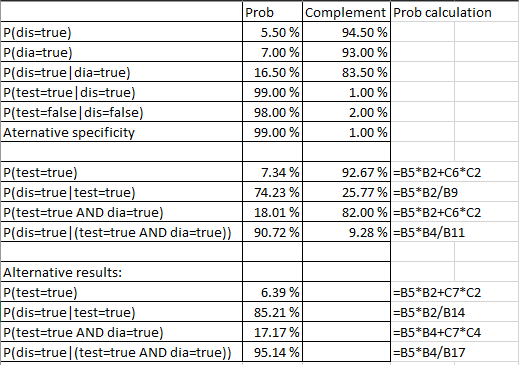
\includegraphics[width=0.9\textwidth]{calc_2.png}
	\caption{The plotted PMF on the left and CDF on the right.}
	\label{fig:calc_2}
\end{figure}
\section{\#3 Joint, conditional and marginal probabilities}
For calculations, refer to Table \ref{tab:my-table}.

\begin{enumerate}[label=\alph*)]
	\item The probabilities can be found from th table. They can be calculated as taking the product of the probability that i numbers of systems are sold with the probability that weather j occurs. E.g. for 0 systems in cold weather we calculate $0.1 \cdot 0.45=0.045=4.5\%$
	\item Since the product of the marginal probabilities  are not the same as the joint probabilites, we can conclude that they are not independent.
	\item The marginal probabilities can be seen from the PMF column in the table
	\item The plots can be seen from Figure \ref{fig:plots}. The probability of at least three systems is 66.55\%
\end{enumerate}

\begin{table}[H]
	\centering
	\caption{Table of joint probabilities, marginal probabilities (in column PMF) and the cumulative distribution function (CDF)}
	\label{tab:my-table}
	\begin{tabular}{l|l|l|l|l|l|l|}
		\cline{2-7}
		& Cold    & Cool    & Warm     & Hot      & PMF      & CDF       \\ \hline
		\multicolumn{1}{|l|}{0} & 4.50 \% & 2.50 \% & 2.00 \%  & 0.00 \%  & 9.00 \%  & 9.00 \%   \\ \hline
		\multicolumn{1}{|l|}{1} & 2.50 \% & 7.50 \% & 4.00 \%  & 1.25 \%  & 15.25 \% & 24.25 \%  \\ \hline
		\multicolumn{1}{|l|}{2} & 1.50 \% & 7.50 \% & 10.00 \% & 2.50 \%  & 21.50 \% & 45.75 \%  \\ \hline
		\multicolumn{1}{|l|}{3} & 0.80 \% & 3.75 \% & 10.00 \% & 6.25 \%  & 20.80 \% & 66.55 \%  \\ \hline
		\multicolumn{1}{|l|}{4} & 0.50 \% & 2.50 \% & 10.00 \% & 11.25 \% & 24.25 \% & 90.80 \%  \\ \hline
		\multicolumn{1}{|l|}{5} & 0.20 \% & 1.25 \% & 4.00 \%  & 3.75 \%  & 9.20 \%  & 100.00 \% \\ \hline
	\end{tabular}
\end{table}

\begin{figure}
	\centering
	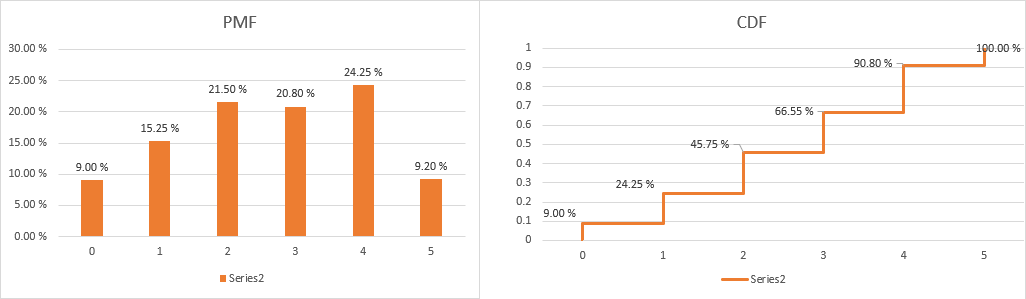
\includegraphics[width=0.9\textwidth]{plots.png}
	\caption{The plotted PMF on the left and CDF on the right.}
	\label{fig:plots}
\end{figure}

\end{document}